\documentclass[border=10pt]{standalone}
\usepackage[T1]{fontenc}
\usepackage{lmodern}
\usepackage[dvipsnames]{xcolor}
\usepackage{tikz}
\usetikzlibrary{positioning,arrows.meta,fit,backgrounds,calc}

\begin{document}
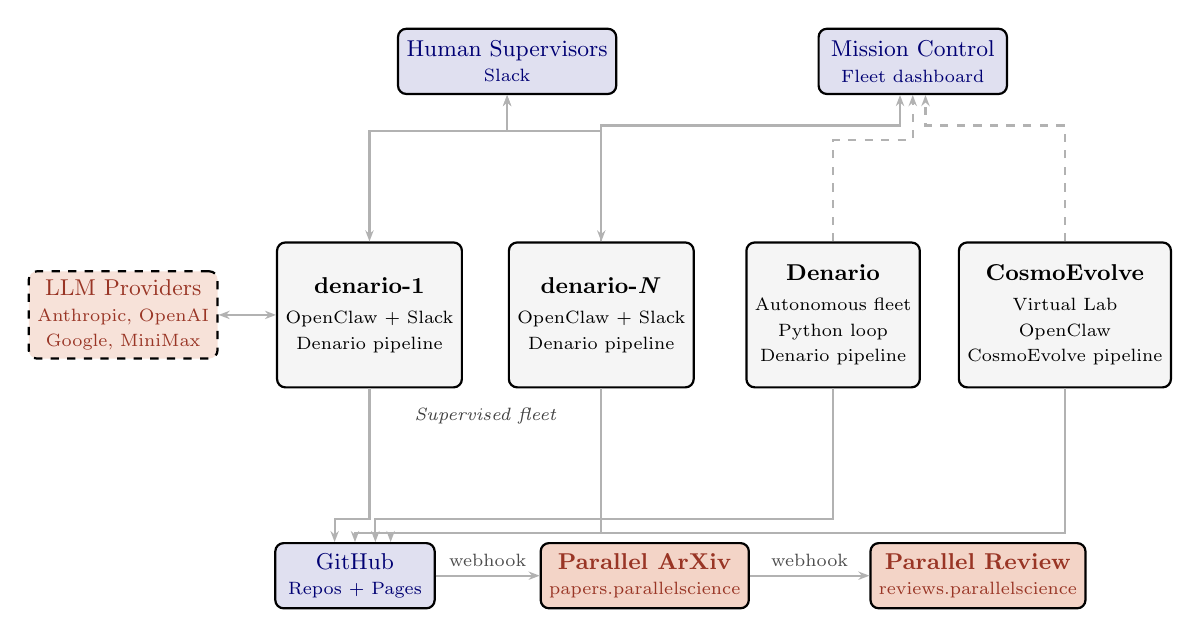
\begin{tikzpicture}[scale=0.92, every node/.style={transform shape},
  box/.style={draw, rounded corners=3pt, minimum height=0.9cm, font=\small, align=center, thick},
  service/.style={box, fill=NavyBlue!12, text=NavyBlue!90!black},
  scientist/.style={box, fill=gray!8, text=black, minimum width=2.3cm, minimum height=2.0cm},
  fleetbox/.style={draw, rounded corners=6pt, dashed, thick, inner xsep=10pt, inner ysep=8pt},
  external/.style={box, fill=BrickRed!10, text=BrickRed!80!black, dashed},
  arr/.style={-{Stealth[length=4pt]}, thick, gray!60},
  darr/.style={{Stealth[length=4pt]}-{Stealth[length=4pt]}, thick, gray!60},
]

% === Scientists ===
\node[scientist] (d1) at (0, 0) {
  \textbf{denario-1}\\[1pt]
  {\scriptsize OpenClaw + Slack}\\[-1pt]
  {\scriptsize Denario pipeline}
};
\node[scientist] (dN) at (3.2, 0) {
  \textbf{denario-\textit{N}}\\[1pt]
  {\scriptsize OpenClaw + Slack}\\[-1pt]
  {\scriptsize Denario pipeline}
};
\node[scientist] (da) at (6.4, 0) {
  \textbf{Denario}\\[1pt]
  {\scriptsize Autonomous fleet}\\[-1pt]
  {\scriptsize Python loop}\\[-1pt]
  {\scriptsize Denario pipeline}
};
\node[scientist] (ce) at (9.6, 0) {
  \textbf{CosmoEvolve}\\[1pt]
  {\scriptsize Virtual Lab}\\[-1pt]
  {\scriptsize OpenClaw}\\[-1pt]
  {\scriptsize CosmoEvolve pipeline}
};

% Fleet label (below supervised only)
\node[font=\scriptsize\itshape, text=gray!50!black] at (1.6, -1.4) {Supervised fleet};

% === Human supervisors (top left) ===
\node[service, minimum width=2.8cm] (human) at (1.9, 3.5) {Human Supervisors\\[-1pt]{\scriptsize Slack}};

% === Mission Control (top right) ===
\node[service, minimum width=2.6cm] (dash) at (7.5, 3.5) {Mission Control\\[-1pt]{\scriptsize Fleet dashboard}};

% === LLM providers (left) ===
\node[external, minimum width=2.4cm] (llms) at (-3.4, 0) {LLM Providers\\[-1pt]{\scriptsize Anthropic, OpenAI}\\[-1pt]{\scriptsize Google, MiniMax}};

% === GitHub (bottom left) ===
\node[service, minimum width=2.2cm] (gh) at (-0.2, -3.6) {GitHub\\[-1pt]{\scriptsize Repos + Pages}};

% === Parallel ArXiv (bottom center) ===
\node[box, fill=BrickRed!15, text=BrickRed!80!black] (pax) at (3.8, -3.6) {\textbf{Parallel ArXiv}\\[-1pt]{\scriptsize papers.parallelscience}};

% === Parallel Review (bottom right) ===
\node[box, fill=BrickRed!15, text=BrickRed!80!black] (prv) at (8.4, -3.6) {\textbf{Parallel Review}\\[-1pt]{\scriptsize reviews.parallelscience}};

% === Arrows ===
% Human <-> supervised scientists
\draw[darr] (human.south) -- ++(0,-0.5) -| (d1.north);
\draw[darr] (human.south) -- ++(0,-0.5) -| (dN.north);

% Dashboard: solid from supervised, dashed from others
\draw[arr] (dN.north) -- ++(0,1.6) -| ([xshift=-5pt]dash.south);
\draw[arr, dashed] (da.north) -- ++(0,1.4) -| ([xshift=0pt]dash.south);
\draw[arr, dashed] (ce.north) -- ++(0,1.6) -| ([xshift=5pt]dash.south);

% LLMs
\draw[darr] (llms.east) -- (d1.west);

% Scientists -> GitHub
\draw[arr] (d1.south) -- ++(0,-1.8) -| ([xshift=-8pt]gh.north);
\draw[arr] (dN.south) -- ++(0,-2.0) -| ([xshift=0pt]gh.north);
\draw[arr] (da.south) -- ++(0,-1.8) -| ([xshift=8pt]gh.north);
\draw[arr] (ce.south) -- ++(0,-2.0) -| ([xshift=14pt]gh.north);
\draw[arr] (gh.east) -- node[above, font=\scriptsize, text=gray!60!black, pos=0.5] {webhook} (pax.west);
\draw[arr] (pax.east) -- node[above, font=\scriptsize, text=gray!60!black, pos=0.5] {webhook} (prv.west);

\end{tikzpicture}
\end{document}
